\documentclass{article}
\usepackage{authblk}
\usepackage{amsmath}
\usepackage{todonotes}
\usepackage{amssymb}
\usepackage{subcaption}
\usepackage[normalem]{ulem}
\usepackage{graphicx}
\usepackage{cite}
\usepackage{marginnote}
\usepackage[colorlinks=true,urlcolor=blue,citecolor=red,linkcolor=red,bookmarks=true]{hyperref}
%strikethrough
\usepackage{soul}
\usepackage{pgfplots}
\pgfplotsset{compat=1.14}
\usepackage{float}
\usepackage[margin=0.5in]{geometry}


\newcommand{\fp}{P_{\text{fp}}}
\newcommand{\fn}{P_{\text{fn}}}
\newcommand{\Se}{S_e}
\newcommand{\Sp}{S_p}
\newcommand{\mi}{P_{\text{sfn}}}
\newcommand{\rel}{E_{\text{rel}}}
\renewcommand\Affilfont{\itshape\small}
\renewcommand{\Pr}{\mathbb{P}}


\begin{document}

\title{Inflated false-negative rates in pooled RT-PCR tests of SARS-CoV-2}


\author[1,2]{Yair Daon, PhD}
\author[2,3]{Amit Huppert, PhD}
\author[1,2]{Uri Obolski, PhD}

\affil[1]{Porter School of the Environment and Earth Sciences, The Faculty of Exact Sciences, Tel Aviv
  University\\ Tel Aviv, Israel}
\affil[2]{School of Public Health, The Faculty of Medicine, Tel Aviv University\\ Tel Aviv, Israel}
\affil[3]{The Gertner Institute for Epidemiology and Health Policy Research, Tel Hashomer, Israel}
%\email{yair.daon@gmail.com}
\date{\today}

\maketitle
%%% MAKE TITLE PAGE %%%
% \bigskip
% \bigskip
% \bigskip
% \bigskip
% \begin{itemize}
%     \item Article type: Brief report.
%     \item Corresponding author: Uri Obolski, email uriobols@tauex.tau.ac.il, Phone +972526309508
%     \item Running head: Inflated false-negative rates in pooled SARS-CoV-2 tests.
%     \item Conflict of interests: None.
%     \item Financial support: Yair Daon was supported by a
%     post-doctoral fellowship from the Tel Aviv University Center for
%     Combating Pandemics and the Raymond and Beverly Sackler Dean's
%     Post-Doctoral fellowship.
%     \item Data is presented in the manuscript itself and can be found in a paper we reference to. Calculations are simple and can be easily implemented in any programming language.
% \end{itemize}
% \end{document}

\begin{abstract}
\textbf{Background}: Pooling is a popular strategy for increasing SARS-CoV-2 testing throughput. One popular pooling scheme is Dorfman pooling: test $N$ individuals simultaneously. If the test is positive --- retest each individual separately. However, requiring more than one positive test may lead to increased false-negative rates.

\textbf{Methods}: We analyze the false-negative rate (i.e., the probability of a negative result for an infected individual) of Dorfman pooling via a new probabilistic model. We demonstrate that different, previously made probabilistic assumptions regarding pooling are unlikely in light of empiric data. Our model is conservative in that it ignores sample dilution effects, which can only worsen pooling performance.

\textbf{Results}: We show that one can expect a 60-80\% increase in false-negative rates under Dorfman pooling, for reasonable parameter values. Moreover, we show that the false-negative rates under Dorfman pooling increase when the prevalence of infection decreases.

\textbf{Discussion}: In most pooling schemes, identifying an infected individual requires positive results in multiple tests and hence substantially increases false-negative rates. Furthermore, this phenomenon is more pronounced when infection prevalence is low --- exactly when pooling is most efficient. Thus, pooling presents an inherent trade-off: it is most efficient when it is least accurate. The deterioration of false-negative rates and the aforementioned trade-off are inherent problems of pooling schemes and should be kept in mind by practitioners and policy makers.
\end{abstract}

\section{Introduction}

RT-PCR testing is a key component in breaking transmission chains and mitigating the COVID-19 pandemic. As such, the need for large-scale testing has resulted in the development of pooling schemes of RT-PCR tests \cite{DorfmanYuvalDor, PoolSize30, BayesianDorfman, MatrixPooling, LionDorfman}. One such popular scheme is Dorfman pooling \cite{DorfmanOriginal, DorfmanYuvalDor}: Select $N$ individuals and perform a single RT-PCR test on their combined (``pooled'') samples. If the pooled test yields a positive result --- test each individual separately. The throughput efficiency of Dorfman pooling has been demonstrated empirically \cite{DorfmanYuvalDor}. However, when test error rates are taken into consideration, a sharp increase in false-negative rates can be expected. 

It is important to distinguish three types of false-negative events when performing pooling. For convenience, we follow a single \emph{infected} individual, henceforth referred to as "Donald". A \emph{single test's} false-negative is the event of a negative result upon testing Donald separately, i.e., in an RT-PCR test without pooling. We denote the test sensitivity $\Se$, so the probability of a single test false-negative is $1-\Se$. A \emph{pooled} false-negative occurs when a pooled test containing Donald's sample (and other samples) yields a negative result, i.e., the pooling fails to detect at least one positive result. Lastly, a \emph{scheme} false-negative occurs when an entire pooling scheme fails to identify Donald as infected. Our goal is to calculate Dorfman's scheme false-negative rate. Rephrasing, we wish to answer the following question: what is the probability of not identifying Donald as infected under a Dorfman pooling scheme? 




\section{Methods}
\subsection{Probabilistic Assumptions}\label{subsec:assumptions}
We assume two pathways for a positive pooled test result: Viral RNA from an infected individual is correctly detected; or, some erroneous detection occurs (e.g. contaminant viral RNA is introduced). We ignore cross-reactivity with other Coronaviruses, which is negligible \cite{KitComparison}. We assume a homogeneous and disconnected population (each individual is infected independently and with equal probability). For simplicity, we do not take into account sample dilution, since it can only further increase false-negative rates \cite{DorfmanYuvalDor}.

Our assumptions, although natural, stand in contrast to assumptions commonly made in the literature \cite{Kim, Simplistic1, Simplistic2, OptimalDorfmanPool}. It is commonly assumed that the probability of a positive pooled test is not increased by having more than one infected individual in the pool. We refute the common assumptions with experimental data summarized in table \ref{table}, collected from \cite{Salazar}. There, the authors investigate Dorfman pooling and, regardless of the pooled test result, follow up and test each pool member separately. Here, we focus on 128 pools for which at least one subsequent separate test was positive --- of which 29 pooled tests were negative and 99 positive. In the data cited in \cite{Salazar}, of the 29 negative pools, subsequent separate testing yielded a single positive result in 24. In contrast, of the 99 positive pools, 42 yielded a single positive test upon subsequent separate testing. 

The data in table \ref{table} allows us to test the following null hypothesis $H_0$: The probability of a pooled false-negative is equal for pools with one subsequent positively tested member and pools with two or more such members. We apply Fisher's exact test for the presence of more than one positive individual in correctly identified pools. Fisher's test yields an increased odds ratio of 6.4, 95\% CI (2.2,23.4), with a p-value $\approx 10^{-4}$. Thus we reject $H_0$, refuting the independence of a pooled result from one or more individuals infected within the pool, as assumed in \cite{Simplistic1, Simplistic2, OptimalDorfmanPool, Kim}

\begin{table}[h]
\centering
\begin{tabular}{ c c c }
                                & Negative pool  & Positive pool \\%& Row total \\ 
\# subsequent positives $=1$    & 24             & 42            \\%& 66        \\  
\# subsequent positives $\geq1$ & 5              & 57            \\%& 62        \\
 Total                          & 29             & 99            \\%& 128 
\end{tabular}
\caption{Contingency table of data from \cite{Salazar}}\label{table}
\end{table}


\subsection{calculation of Dorfman's scheme false-negative rate}\label{subsec:detailed}
Denote the prevalence of infection in the (tested) population $q$. As before, $\Se$ is the test's sensitivity, so $1-\Se$ is the single RT-PCR test's false-negative rate. We also denote $\Sp$ the test specificity --- the true-negative probability. This encompasses events of an erroneous RNA detection (via any possible pathway), which may cause a false-positive. By our assumptions, a pool containing Donald's sample and $N-1$ other samples will yield a \emph{negative} result if all of the following occur: 
\begin{itemize}
\item No erroneous detection occurred (i.e. no false-positive). This happens with probability $\Sp$.
\item The detection process fails for Donald's sample. A false-negative occurs for Donald, with probability $1-\Se$.
\item No detection for any of the other $N-1$ samples. For a single sample, the probability of being detected is the prevalence of SARS-CoV-2 in the tested population $q$, multiplied by the sensitivity $\Se$, hence the probability of detection is $q\Se$. For $N-1$ such samples, the probability of \emph{not} being identified is $(1-q\Se)^{N-1}$. 
\end{itemize}
The pooled false-negative probability for Donald is simply the product of the terms above. Hence:

\begin{align}
    \begin{split}
        \Pr(\text{pool is positive}) &= 1 - \Pr(\text{pool false-negative}) \\
        &= 1 - \Sp(1-\Se)(1-q\Se)^{N-1}.
    \end{split}
\end{align}

If the pooled test yields a positive result, Donald is tested separately. We assume such a simple procedure poses no risk of introducing contaminant RNA. Therefore, the separate test yields a positive result with probability $\Se$. 

We calculate the probability that Donald is mistakenly identified as not infected --- the scheme's false-negative rate --- denoted $\mi$ below. To \emph{correctly} identify Donald as infected, both pooled and separate tests have to yield a positive result. Thus, the scheme's false-negative rate $\mi$ is the complement of the product of the two previous terms:
\begin{align}\label{eq:sfn}
    \begin{split}
        \mi :&= 1-\Pr(\text{correctly identify Donald as infected})\\
        %
        &= 1 - \Se\left [1 - \Sp(1-\Se)(1-q\Se))^{N-1}\right].
    \end{split}
\end{align}

\subsection{Comparison metric}
The single test false-negative rate $1-\Se$ and scheme false-negative rate $\mi$ are compared via:
\begin{equation}\label{eq:erel}
\rel := \frac{\mi - (1-\Se)}{1-\Se} \cdot 100.
\end{equation}
$\rel$ is the percentage increase in the pooling scheme false-negative rate, relative to the single test false-negative rate.

For the approximation commonly used in the literature estimates the scheme false-negative rate as $1-\Se^2$ (section \ref{section:ass} and \cite{Simplistic1, Simplistic2, Kim, OptimalDorfmanPool}). A short calculation shows that this approximation implies the percentage increase in scheme false-negative rate is just $100\cdot \Se$.

\section{Results}\label{section:results}

We plot $\rel$ for varying prevalence $q$ and sensitivity $\Se$ values. As recommended by \cite{DorfmanYuvalDor}, we apply different pool sizes $N$, for different prevalence values. We observe that for a false-positive rate $\Sp=0.95$ \cite{DorfmanYuvalDor} and a range of reasonable sensitivity and prevalence values \cite{KitComparison, InterpretingCOVID19Test, EstimatingRatesLourenco, FalsePositiveEstimate}, an increase of at least $60\%$ in $\rel$ can be expected (Figure \ref{figy}). Interestingly, an increase in infection prevalence monotonically decreases the scheme false-negative rate, as can also be easily seen from equation \eqref{eq:sfn}. For the chosen parameter ranges, the increase in the single test false-negative rates increases the relative error $\rel$. These effects can be seen in Figure \ref{figy} (left panel), upon conditioning on pool size. Extending the range for $\Sp$ yields no qualitative differences. We further compare $\rel$ to the commonly used approximation, showing the discrepancy changes as a function of both prevalence and the single test sensitivity (Figure \ref{figy}, right panel)   
\begin{figure}[H]
    \centering
    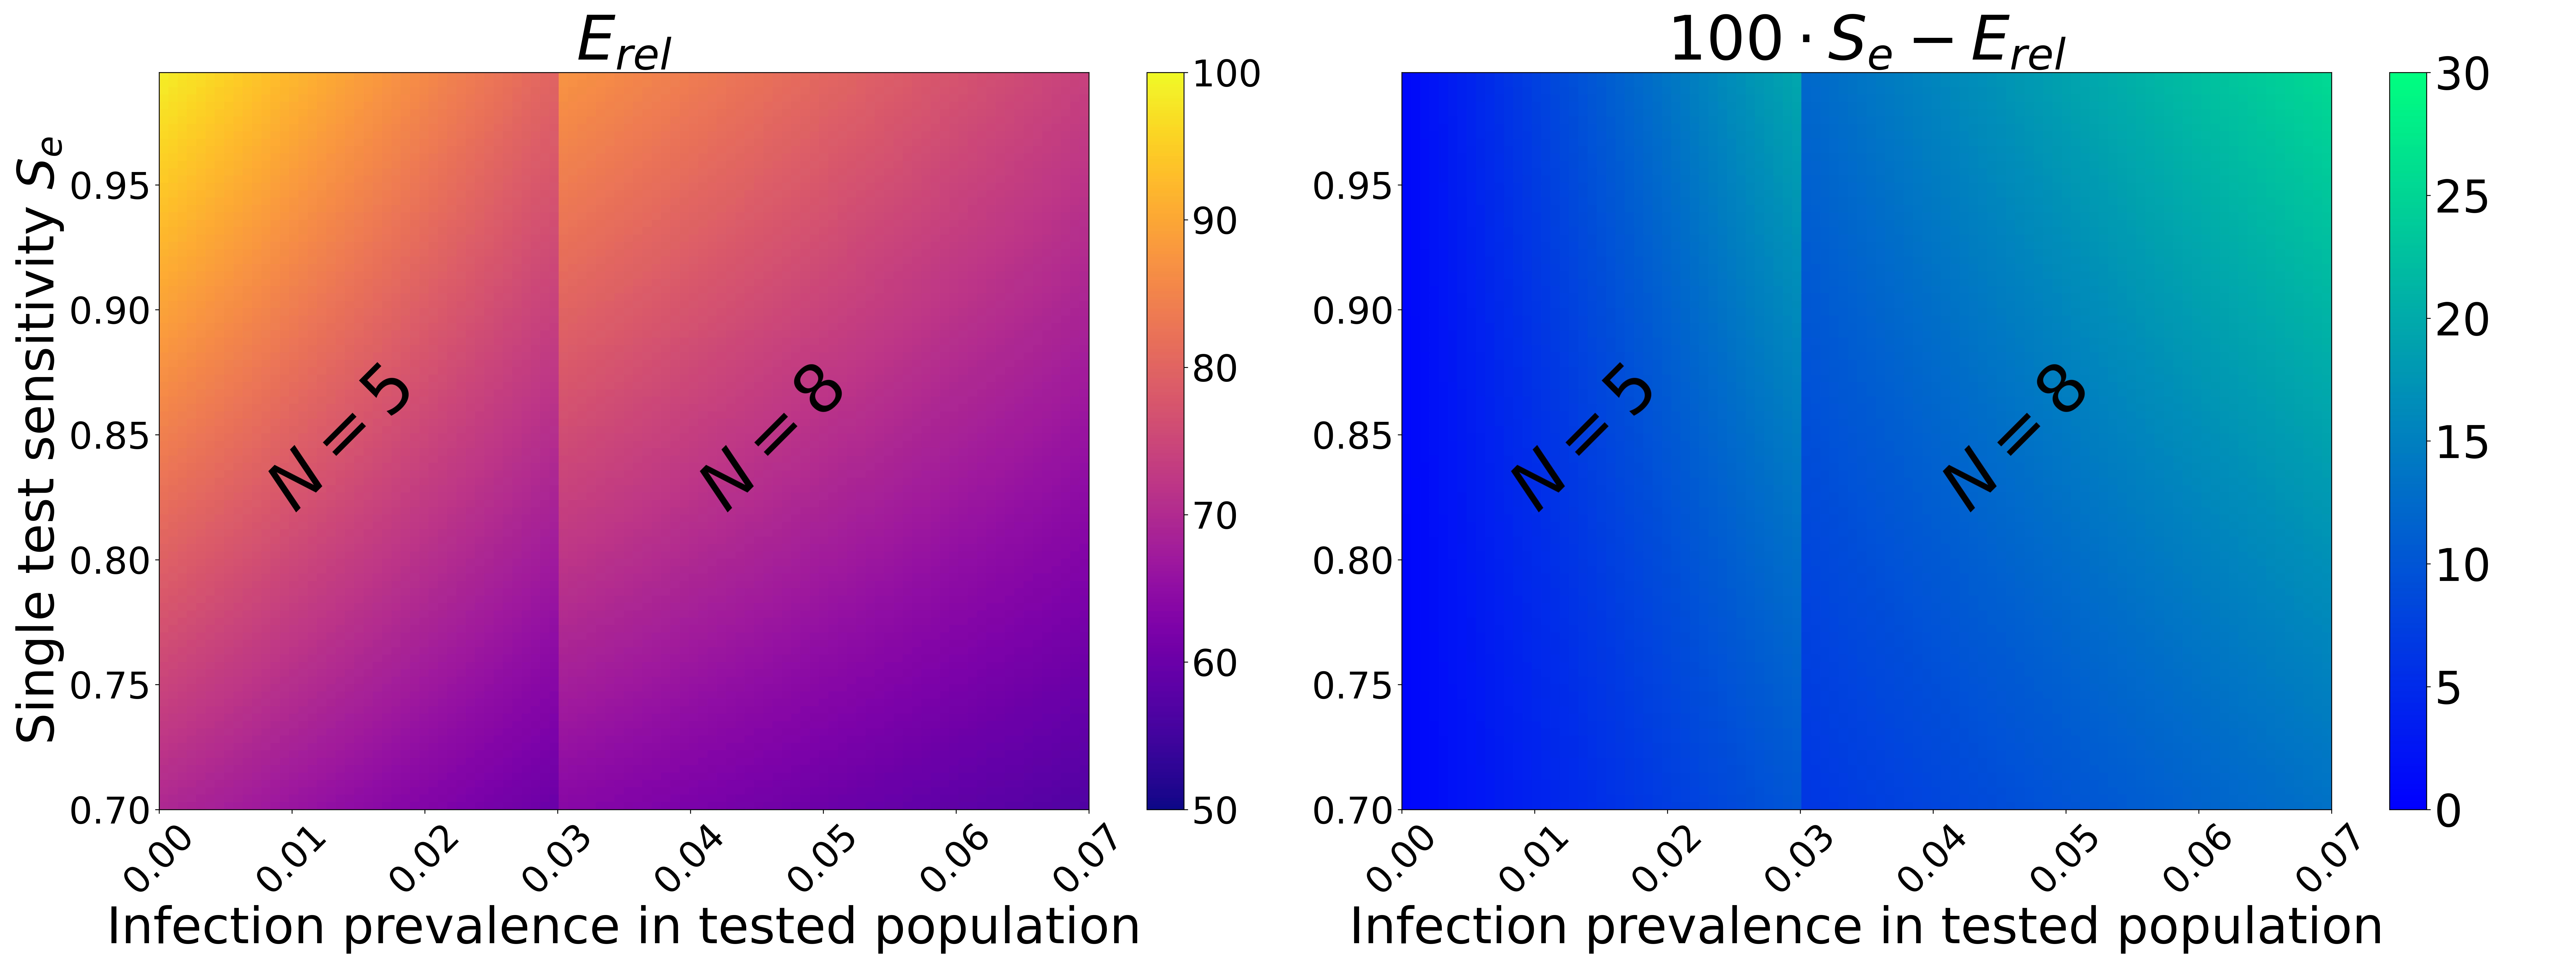
\includegraphics[width=18cm]{heatmap.jpg}
    \caption{Relative increase in Dorfman pooling false-negative rates $\rel$. Left: Colors represent $\rel$, the relative percentage increase in the scheme false-negative rates relative to the single test false-negative rates (eq \eqref{eq:erel}). Right: colors represent the difference between the approximation assumed in other studies and $\rel$ as calculated by our model. The disease prevalence $q$, is varied on the x-axis, while the test sensitivity is varied on the y-axis. Pool size $N$, was chosen according to $q$ as in \cite{DorfmanYuvalDor}.}\label{figy}
 \end{figure}


\section{Discussion}
Although Dorfman pooling improves testing throughput, we have shown that it can increase $\rel$ --- the false-negative rates relative to individual testing. Furthermore, low values of infection prevalence, or low values of single test false-negative rates, increase $\rel$. These results remain qualitatively similar under varying parameter values, in the observed ranges \cite{KitComparison,EstimatingRatesKucrika, EstimatingRatesLourenco, InterpretingCOVID19Test} (Figure \ref{figy}). 

Our results lead to a fact almost disregarded in \cite{DorfmanYuvalDor}: although (Dorfman) pooling is most efficient when prevalence is low, such circumstances are exactly those leading to a substantial increase in false-negative rates. 

An approximation to our results has been previously considered: $\mi \approx 1-\Se^2 $\cite{Simplistic1, Simplistic2, Kim, OptimalDorfmanPool}. Such an approximation arises when one assumes that the probability of a false-negative is identical for the pooled and single tests. Although simplistic in nature, this approximation does capture the intuition behind our results: For Donald to be considered negative under Dorfman pooling, he has to test negative twice. In addition to this approximation only being an upper bound \cite{Simplistic2}, it does not account for the effect of infection prevalence on the false-negative rates under Dorfman pooling. Supporting the importance of this effect, such an association between prevalence and the scheme false-negative rate under Dorfman pooling has been empirically noted  \cite{DorfmanYuvalDor}.

Although we have shown the inherent risk of Dorfman pooling, this shortcoming applies to other pooling schemes. Pooling schemes (e.g. \cite{MatrixPooling,Lion, Kim}), require some sequence of positive pooled results to correctly identify Donald as infected. Consider the hierarchical pooling scheme \cite{Lion, Kim}: If the first pool yields a positive result, it is split in two. Then the splitting is repeated until resulting pools are negative or individuals are tested separately. With an initial pool size of 32, Donald will necessarily have to test positive in pools of size 32, 16, 8, 4 and 2, as well as in a single test, for the scheme to correctly identify him as infected. Compare this to the Dorfman scheme that requires a positive test in a pool of size $N=8$, and an additional single positive test to identify Donald as infected. The hierarchical pooling scheme of \cite{Lion, Kim} will necessarily yield  more false-negatives than Dorfman pooling --- there are additional places for it to fail.

As mentioned in \cite{DorfmanYuvalDor}, introducing a positive dependence within a pool decreases the false-positive rate. In the extreme case, consider a fully connected pool, where one infection implies the entire pool is infected. In this case, a calculation analogous to the one conducted above recovers the initial false-negative rate $1-\Se$. Interestingly, pooling was also noted to have increased throughput when infection probabilities are dependent between the pooled individuals \cite{DorfmanYuvalDor}, providing  another advantage to sampling dependent individuals in pooling schemes.  

To conclude, pooling is an important technique which can improve testing throughput in a cost-effective manner. Nevertheless, a substantial increase in pooling schemes' false-negative rates can be expected. Such a increase has crucial implications for controlling the spread of COVID-19.




\bibliographystyle{ama}
\bibliography{refs}

\end{document}
